%
% Report -- Verilog-A Macromodel for Operational Amplifiers
%
% Copyright (C) 2007 Mike Brinson <mbrin72043@yahoo.co.uk>
%
% Permission is granted to copy, distribute and/or modify this document
% under the terms of the GNU Free Documentation License, Version 1.1
% or any later version published by the Free Software Foundation.
%

% redefine subfigure caption
\renewcommand{\thesubfigure}{\thefigure(\alph{subfigure})}
\makeatletter
  \renewcommand{\@thesubfigure}{\thesubfigure:\space}
  \renewcommand{\p@subfigure}{}
\makeatother

% redefine subtable caption
\renewcommand{\thesubtable}{\thetable(\alph{subtable})}
\makeatletter
  \renewcommand{\@thesubtable}{\thesubtable:\space}
  \renewcommand{\p@subtable}{}
\makeatother

\tutsection{Introduction}

Since the release of Qucs version 0.0.11 the Qucs team has spent a lot
of time and effort improving and debugging the Qucs device and circuit
modelling facilities. Initially, the primary device and circuit
modelling technique available to users was based on a subcircuit
approach that allowed new models to be formed from the built in
components distributed with each release of the package\footnote{It is
also possible to construct models directly in C++ and compile and link
them to the main body of the Qucs code.  This is the approach taken by
the package developers.  However, for the average Qucs user who is
primarily interested in using the package, rather than taking part in
it's development, this route to model development is not really an
option.}.  Releases 0.0.11 and 0.0.12 added model construction centred
around the nonlinear equation defined device (EDD) and ADMS compact
device models.  For these modelling techniques preliminary
documentation and application information has been posted on the Qucs
Web site\footnote{Mike Brinson, ``Qucs Tutorial: Component, compact
device and circuit modelling using symbolic equations``,
\url{http://qucs.sourceforge.net/docs.html}, and Stefan Jahn, H\'{e}l\`{e}ne
Parruitte, ``Qucs Description: Verilog-AMS interface'',
\url{http://qucs.sourceforge.net/docs.html}.}, outlining the fundamental
basis of these procedures.  Unfortunately, both the EDD and ADMS
modelling techniques do require a level of specialised knowledge which
many Qucs users may be unfamiliar with. These notes have been written
in the hope that the information they provide will help add to the
body of information published on Qucs modelling and also be useful to
other Qucs users who would like to try constructing, and experimenting
with, new device and circuit models using the ADMS software. Today
Qucs has moved on from simply a GPL circuit simulator with user
friendly schematic capture, and has started to evolve into an advanced
circuit and device modelling tool which offers features that were not
commonly available in previous generations of GPL circuit simulators.
This report introduces an ADMS synthesised compact macromodel for the
modular operational amplifier previously described in the Qucs
tutorial on operational amplifiers.\footnote{Mike Brinson, ``Qucs
Tutorial: Modelling Operational Amplifiers'',
\url{http://qucs.sourceforge.net/docs.html}.}. This macromodel is
characterised by a similar symbol to the primitive operational
amplifier gain block included with all Qucs releases.  However, it
provides Qucs with a more realistic general purpose operational
amplifier model that can be used with confidence when designing many
practical circuits which are dependent on amplifier characteristics
for correct operation. The process of compiling and linking ADMS
generated C++ models with the Qucs C++ code has been a learning
vehicle on my part, allowing some of the complexities of the ADMS
Verilog-A compiler to be decoded and understood.  The ADMS synthesised
operational amplifier macromodel also marks a departure from the
previously described Qucs compact device models in that it represents
a circuit function rather than a semiconductor device characteristic.
The source code for the modular macromodel is included in this report
and the ADMS generated C++ code can be found in the Qucs release
source tarballs archive\footnote{Available from
\url{http://qucs.sourceforge.net/download.html}}. The procedure used to
synthesize and link the model to Qucs followed the route suggested by
Stefan and H\'{e}l\`{e}ne in their report on the Verilog-AMS/Qucs
interface.


\tutsection{A Modular Macromodel for an Operational Amplifier}

An introduction to the technical specification and structure of a
modular macromodel for a general purpose operational amplifer is given
on page 7 of the Qucs operational amplifier tutorial. The
characteristics of this operational amplifier macromodel are:

\begin{itemize}
 \item Input stage: Offset voltage and current, bias current, differential resistance and capacitance.
 \item Gain stages: Two pole differential response and single zero common-mode response.
 \item Large signal response: Slew rate limiting.
 \item Output stage: Resistance, output voltage and current limiting.
\end{itemize}

\tutsection{Parameters}

\begin{longtable}{rllll}
Name & Symbol & Description & Unit & Default$^{*}$\\
\hline
\endhead
GBP & $GBP$ & Gain bandwidth product & Hz & 1e6\\
AOLDC & $AOLDC$ & Open-loop differential gain at DC & dB & 106.0\\
FP2 & $FP2$ & Second pole frequency & Hz & 3e6\\
RO & $RO$ & Output resistance & $\ohm$ & 75\\
CD & $CD$ & Differential input capacitance & F & 1e-12\\
RD & $RD$ & Differential input resistance & $\ohm$ & 2e6\\
IOFF & $IOFF$ & Input offset current & A & 20e-9\\
IB & $IB$ & Input bias current & A & 80e-9\\
VOFF & VOFF & Input offset voltage & V & 7e-4\\
CMRRDC & $CMRRDC$ & Common-mode rejection ratio at DC   & dB & 90.0\\
FCM & $FCM$ & Common-mode zero corner frequency & Hz  & 200.0\\
PSRT & $PSRT$ & Positive slew rate & V/s & 5e5\\
NSRT & $NSRT$ & Negative slew rate & V/s & 5e5\\
VLIMP & $VLIMP$ & Positive output voltage limit & V & 14\\
VLIMN & $VLIMPN$ & Negative output voltage limit & V & -14\\
ILMAX & $ILMAX$ & Maximum output current at DC & A & 35e-3\\
CSCALE & $CSCALE$ & Current limit scale factor &   & 50\\
\end{longtable}

* The default parameters are for a typical UA741 Operational Amplifier.


\tutsection{Verilog-A model code}

\begin{lstlisting}[
 language=Verilog, 
 xleftmargin=12pt,
 basicstyle=\scriptsize]
//   Qucs modular OP AMP model:
//   Default parameters are for a typical UA741.
//
// This is free software; you can redistribute it and/or modify
// it under the terms of the GNU General Public License as published by
// the Free Software Foundation; either version 2, or (at your option)
// any later version.
// 
// Copyright (C), Mike Brinson, mbrin72043@yahoo.co.uk, November 2007.
//
`include "disciplines.vams"
`include "constants.vams"
// 
 module mod_amp (in_p, in_n, out_p);
 inout in_p, in_n, out_p;
 electrical in_p, in_n, out_p;
 electrical n2, n3, n4, n5, n6, n7, n8, n9, n10, n11, n12;
//   
 `define attr(txt) (*txt*)
//
 parameter real GBP =1e6 from [1 : inf]
  `attr(info="Gain bandwidth product (Hz)");
 parameter real AOLDC = 106.0 from [0.01 : inf] 
  `attr(info="Open loop DC gain (dB)");
 parameter real FP2 = 3e6 from [0.01 : inf]
  `attr(info="Second pole frequency (Hz)");
 parameter real RO = 75 from [0.01 : inf]
  `attr(info="Output resistance (Ohm)");
 parameter real CD = 1e-12 from [1e-20 : inf]
  `attr(info="Differential input capacitance (F)");
 parameter real RD = 2e6 from [0.01 : inf]
  `attr(info="Differential input resistance (Ohm)");
 parameter real IOFF = 20e-9 from [1e-20 : inf]
  `attr(info="Input offset current (A)");
 parameter real IB = 80e-9 from [1e-20 : inf]
  `attr(info="Input bias current (A)");
 parameter real VOFF = 7e-4 from [0 : inf]
  `attr(info="Input voltage offset (A)");
 parameter real CMRRDC = 90.0 from [1 : inf]
  `attr(info="Common mode rejection ratio at DC (dB)");
 parameter real FCM = 200 from [0.01 : inf]
  `attr(info="Common mode zero corner frequency (Hz)");
 parameter real PSRT = 5e5 from [1 : inf]
  `attr(info="Positive slew rate (V/s)");
 parameter real NSRT = 5e5 from [1 : inf]
  `attr(info="Negative slew rate (V/s)");
 parameter real VLIMP = 14 from [0.01 : inf]
  `attr(info="Positve output voltage limit (V)");
 parameter real VLIMN = -14 from [-inf : 0]
  `attr(info="Negative output voltage limit (V)");
 parameter real ILMAX = 35e-3 from [1e-9 : inf]
  `attr(info="Maximum DC output current (A)");
 parameter real CSCALE = 50 from [0 : inf]
  `attr(info="Current limit scaling factor");
// 
 real RP1, CP1, RP2, CP2;
 real Rdiff,  Voffset;
 real CMRR0, CMgain, CCM; 
 real Slewratepositive, Slewratenegative;
 real MTWOPI;
//
 analog begin
//
// Constants
//
   MTWOPI =  6.28318530717958647693;
//
// Design equations
//
   Voffset = VOFF*5;
   Rdiff = RD/2;
   CMRR0 = pow(10, CMRRDC/20);
   CMgain = 1e6/CMRR0;
   CCM = 1.0/(MTWOPI*1e6*FCM);
   RP1 = pow(10, AOLDC/20);
   CP1 = 1/(MTWOPI*GBP);
   RP2 = 1;
   CP2 = 1/(MTWOPI*FP2);
   Slewratepositive = PSRT/(MTWOPI*GBP);
   Slewratenegative = NSRT/(MTWOPI*GBP);
//
// Input voltage offset
//
    I(in_p, n7) <+ V(in_p, n7);
    I(in_p, n7) <+ Voffset;
//
    I(in_n, n9) <+ V(in_n, n9);
    I(in_n, n9) <+ -Voffset;
//
// Input bias currents
//
    I(n7) <+ IB;
    I(n9) <+ IB;
//
// Input current offset
//
    I(n7,n9) <+ IOFF/2;
//
// Input differential resistance and capacitance
//
  I(n7, n8) <+ V(n7, n8)/Rdiff;
  I(n9, n8) <+ V(n9, n8)/Rdiff;
  I(n7, n9) <+ ddt(CD*V(n7, n9));
//
// Common mode stage
//
  I(n6) <+ -CMgain*V(n8);
  I(n6) <+ V(n6);
  I(n6, n10) <+ V(n6, n10)/1e6;
  I(n6, n10) <+ ddt(CCM*V(n6, n10));
  I(n10) <+ V(n10);
//
// Differential mode and common mode signal adder stage
//
   I(n11) <+ -V(n10);
   I(n11) <+ -V(n7, n9);
   I(n11) <+  V(n11);
//
// Slew rate limiting stage
//
   if (V(n11) > Slewratepositive)
                      I(n12) <+ -Slewratepositive;
   else if (V(n11) < -Slewratenegative)
                      I(n12) <+  Slewratenegative;
   else I(n12) <+ -V(n11);

   I(n12) <+ V(n12);
// 
// First pole
//
   I(n3) <+ -V(n12);
   I(n3) <+ V(n3)/RP1;
   I(n3) <+ ddt(CP1*V(n3));
//
// Second pole
//
   I(n5) <+ -V(n3);
   I(n5) <+ V(n5)/RP2;
   I(n5) <+ ddt(CP2*V(n5));
//
// Current limiter stage
//
   if (V(n2, out_p) >= ILMAX) 
      begin
        I(n4) <+  -V(n5);
        I(n4) <+ CSCALE*V(n5)*(V(n2, out_p) - ILMAX);
        I(n4) <+ V(n4);
      end
   else if (V(n2, out_p) <= -ILMAX)
      begin
        I(n4) <+  -V(n5);
        I(n4) <+ -CSCALE*V(n5)*(V(n2, out_p) + ILMAX);
        I(n4) <+ V(n4);
      end
   else
      begin
        I(n4) <+ -V(n5);
        I(n4) <+  V(n4);
      end
//
// Output resistance
//
   I(n4, n2) <+ V(n4, n2)/(RO-1);
   I(n2, out_p) <+ V(n2, out_p);
//
//
// Voltage limiter stage
//
   if (V(out_p) > VLIMP)
      begin
        I(out_p) <+  -10.0*VLIMP;
        I(out_p) <+ 10.0*V(out_p);
      end
  else if (V(out_p) < VLIMN)
      begin
        I(out_p) <+ -10.0*VLIMN;
        I(out_p) <+ 10.0*V(out_p);
     end
  end
  endmodule
\end{lstlisting}

The ADMS syntax is a subset of Verilog-A.  Allowed language structures
are outlined in a SYNTAX-SUPPORTED file which can be downloaed from
\url{http://mot-adms.sourceforge.net}.

\tutsection{Model test examples}

In the following sections a series of test results are presented.
These illustrate how the modular macromodel performs in comparison to
the transistor level\footnote{The UA741 transistor level model can be
found in the Qucs OpAmps component library. } model for the UA741
operational amplifier.  Typical parameters for the UA741 operational
amplifier are listed in the introduction to this report.  These values
have been extracted from UA741 device data sheets provided by
manufacturers.  In the test simulations the modular UA741 parameters
have been adjusted to give similar simulation results obtained from
the transistor level model.  A number of interesting differences
between the simulation results obtained with the modular macromodel,
plus default parameters, and the transistor level model are observed,
for example the transistor level simulation results yield a value for
IOFF of approximately zero amperes.  With a real device this is
unlikely to occur due to mismatches in the input transistor
properties.  In the transistor level model the input transistors are
identical implying perfect matching.  This is, of course, unlikely to
be the case with a real device. Once again the results demonstrate one
of the most important rules in circuit simulation, namely that the
accuracy of the results from a specific simulation does largely depend
on how well a model represents a physical device or circuit.  Further
comments about the Verilog-A code and the accuracy of the simulation
results are given with each set of test results.


\tutsubsection{Input voltage offset}

Input voltage offset is represented by the Verilog-A code listed in
this section.  This models the input voltage offset by two batteries
of value VOFF/2. These are formed by current generators in parallel
with one Ohm resistors.  Notice that the direction of the current
generator current flow determines the polarity of the batteries.


\begin{lstlisting}[
 language=Verilog, 
 xleftmargin=12pt,
 basicstyle=\scriptsize]
// Input voltage offset
//
    I(in_p, n7) <+ V(in_p, n7);
    I(in_p, n7) <+ Voffset;
//
    I(in_n, n9) <+ V(in_n, n9);
    I(in_n, n9) <+ -Voffset;
\end{lstlisting}

 
\begin{figure} [here]
  \centering
  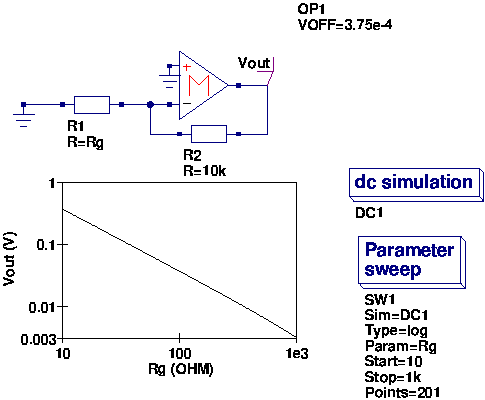
\includegraphics[width=0.6\linewidth]{mod_amp_Fig1}
  \caption{UA741 modular macromodel input voltage offset test circuit and results}
  \label{fig:mod_amp1}
\end{figure} 

\begin{figure} [here]
  \centering
  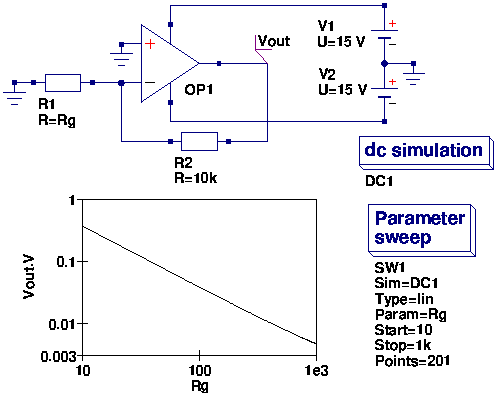
\includegraphics[width=0.6\linewidth]{mod_amp_Fig2} 
  \caption{UA741 transistor level input voltage offset test circuit and simulation results}
  \label{fig:mod_amp2}
\end{figure} 




\tutsection{Input bias and offset currents}

Input bias and offset currents are represented by the Verilog-A code
listed in this section. Simple current generators are employed to
model the input current effects. Values for IB and IOFF can be
extracted from the results given in Figs.~\ref{fig:mod_amp3} and
~\ref{fig:mod_amp4}, using equations (1) and (2).

\begin{flushright}
$Vp=-(IB+\dfrac{IOFF}{2}).1e3$   \hspace{5.5cm}(1)
\linebreak  
$Vn-Vs = (\dfrac{IOFF}{2}-IB).1e3$  \hspace{5cm}(2)
\end{flushright}

 The remainder of the input stage Verilog-A code adds differential
 input resistance and capacitance to the input stage of the
 operational amplifier macromodel.

\begin{lstlisting}[
 language=Verilog, 
 xleftmargin=12pt,
 basicstyle=\scriptsize]
// Input bias currents
//
    I(n7) <+ IB;
    I(n9) <+ IB;
//
// Input current offset
//
    I(n7,n9) <+ IOFF/2;
//
// Input differential resistance and capacitance
//
  I(n7, n8) <+ V(n7, n8)/Rdiff;
  I(n9, n8) <+ V(n9, n8)/Rdiff;
  I(n7, n9) <+ ddt(CD*V(n7, n9));
\end{lstlisting}

\begin{figure} [here]
  \centering
  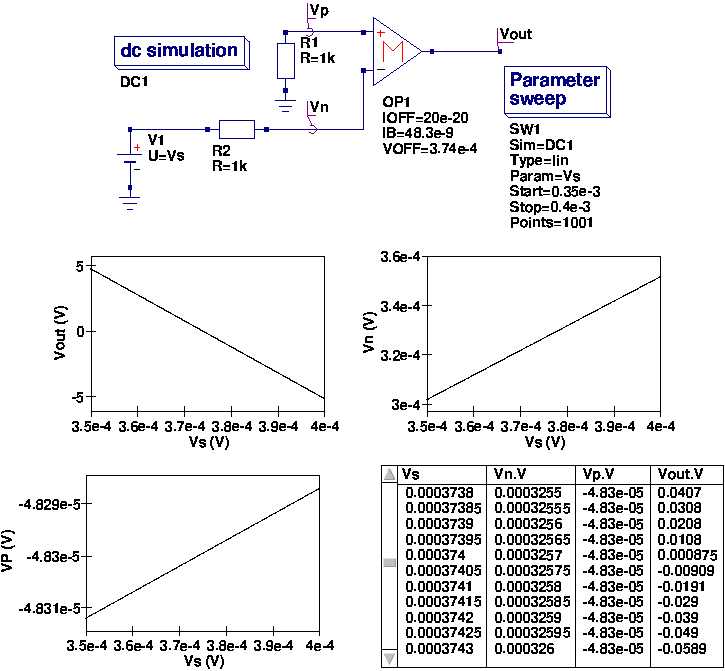
\includegraphics[width=0.75\linewidth]{mod_amp_Fig3}
  \caption{UA741 modular macromodel input bias and offset current test circuit and simulation results}
  \label{fig:mod_amp3}
\end{figure} 

\begin{figure} [here]
  \centering
  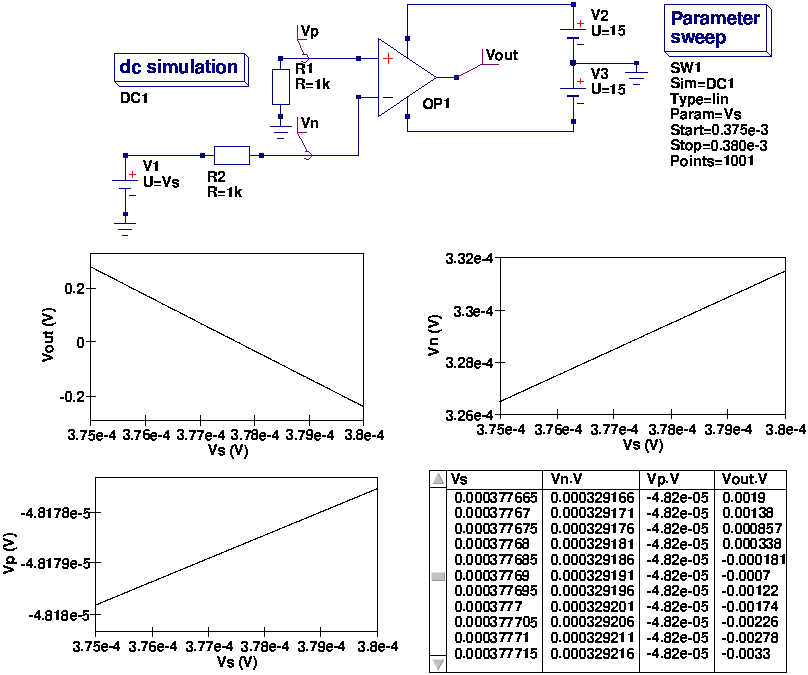
\includegraphics[width=0.75\linewidth]{mod_amp_Fig4}
  \caption{UA741 transistor level input bias and offset current test circuit and simulation results}
  \label{fig:mod_amp4}
\end{figure} 


\tutsection{Open loop differential voltage gain}

Differential voltage gain is represented by the Verilog-A code listed
in this section. Differential gain is modelled with three distinct
quantities. These are 1. resistor RP1 which is set equal to the open
loop differential gain at DC, 2. the primary pole in the voltage gain
frequency response which is set by capacitor CP1, and 3. a high
frequency pole set by CP2 and resistor RP2. Each pole stage is driven
by a voltage controlled current generator. Note the current generator
negative sign. This is required to maintain the correct signal
phase. The derivation, and a more detailed discussion, of the model
open-loop differential voltage gain properties can be found in pages
13 to 19 of the Qucs operational amplifier tutorial. Simulated results
for the open-loop differential gain response are shown in
Figs.~\ref{fig:mod_amp5} and~\ref{fig:mod_amp6} The AOLDC and CD
parameters given in Fig.~\ref{fig:mod_amp5} have been adjusted to give
the same response as the Qucs transistor level model.  Again due to
perfect transistor matching a value of CD roughly zero is required to
produce similar high frequency responses above the second pole
frequency.

\begin{lstlisting}[
 language=Verilog, 
 xleftmargin=12pt,
 basicstyle=\scriptsize]
// 
// First pole
//
   I(n3) <+ -V(n12);
   I(n3) <+ V(n3)/RP1;
   I(n3) <+ ddt(CP1*V(n3));
//
// Second pole
//
   I(n5) <+ -V(n3);
   I(n5) <+ V(n5)/RP2;
   I(n5) <+ ddt(CP2*V(n5));
//
\end{lstlisting}

\begin{figure} [here]
  \centering
  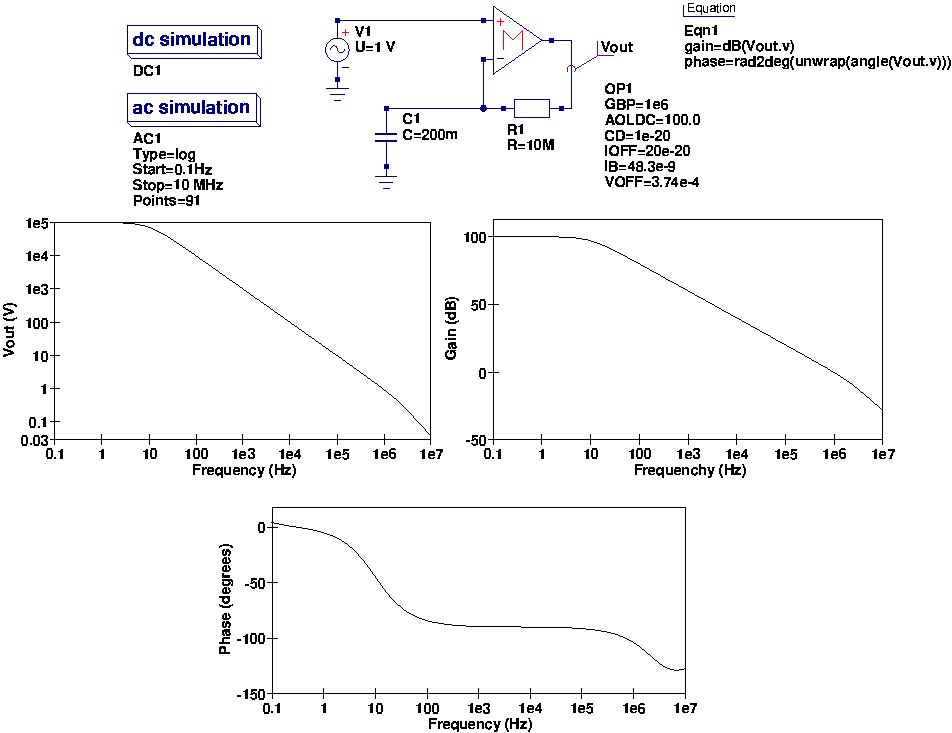
\includegraphics[width=0.8\linewidth]{mod_amp_Fig5}
  \caption{UA741 modular macromodel open-loop differential voltage gain test circuit and simulation results}
  \label{fig:mod_amp5}
\end{figure} 


\begin{figure} [here]
  \centering
  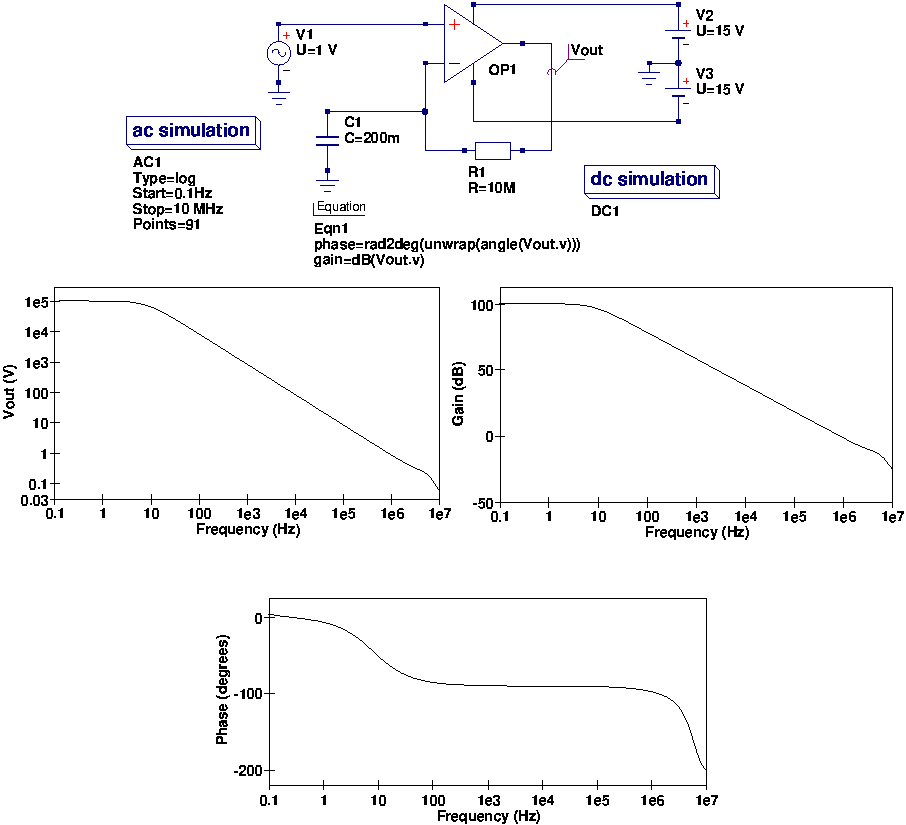
\includegraphics[width=0.8\linewidth]{mod_amp_Fig6}
  \caption{UA741 transistor level open-loop differential voltage gain test circuit and simulation results}
  \label{fig:mod_amp6}
\end{figure} 




\tutsection{Common mode effects}

Operational amplifier common-mode effects are represented by the
Verilog-A code listed in this section. Common-mode effects are
simulated using an identical network to that outlined in page 20 the
Qucs operational amplifier tutorial. The simulated results for a unity
gain CMMR test circuit are illustrated in Figs.~\ref{fig:mod_amp7}
and~\ref{fig:mod_amp8}.  The macromodel parameters CMRR and FCM have
been set at their default values to demonstrate the difference when
compared to the transistor level model. Common-mode simulation results
observed with the transistor level model are significantly better than
those obtained from measurements on real devices, mainly because the
simulation model is constructed from perfectly matched
transistors. Associated with the differential amplifier stages and the
common-mode section of the macromodel is a signal adder which combines
the differential and common-mode signals.  The Verilog code for this
adder stage is also repeated with common-mode code.  An adder can be
formed by a one Ohm resistor driven by differential and common-mode
currents. The resulting volt drop across the one Ohm resistor then
becomes the sum of the two signal voltages.


\begin{lstlisting}[
 language=Verilog, 
 xleftmargin=12pt,
 basicstyle=\scriptsize]
//
// Common mode stage
// 
  I(n6) <+ -CMgain*V(n8);
  I(n6) <+ V(n6);
  I(n6, n10) <+ V(n6, n10)/1e6;
  I(n6, n10) <+ ddt(CCM*V(n6, n10));
  I(n10) <+ V(n10);
//
// Differential mode and common mode signal adder stage
//
   I(n11) <+ -V(n10);
   I(n11) <+ -V(n7, n9);
   I(n11) <+  V(n11);
//
\end{lstlisting}

\begin{figure} [here]
  \centering
  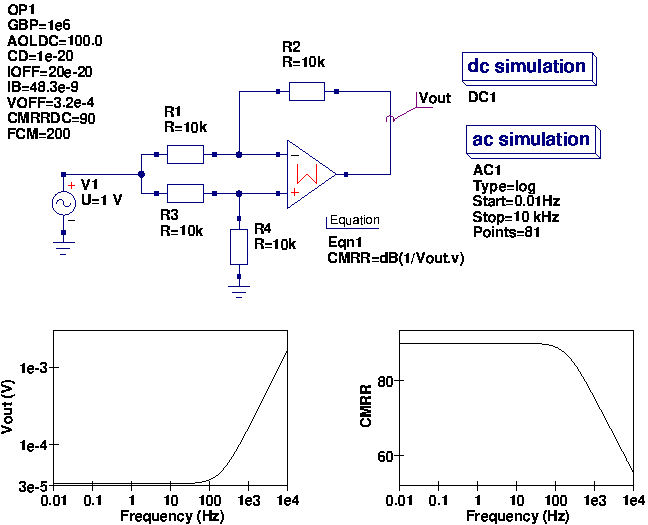
\includegraphics[width=0.6\linewidth]{mod_amp_Fig7}
  \caption{UA741 modular macromodel CMRR test circuit and simulation results}
  \label{fig:mod_amp7}
\end{figure} 


\begin{figure} [here]
  \centering
  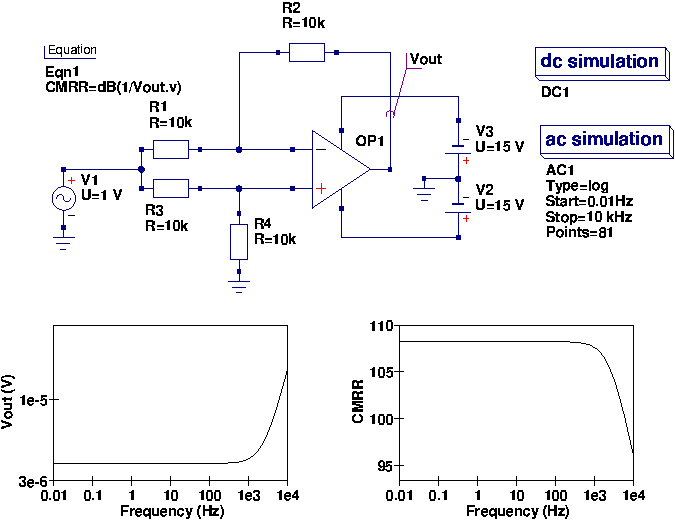
\includegraphics[width=0.6\linewidth]{mod_amp_Fig8}
  \caption{UA741 transistor level CMRR test circuit and simulation results}
  \label{fig:mod_amp8}
\end{figure} 


\tutsection{Slew rate limiting}

Operational amplifier slew rate limiting effects are represented by
the Verilog-A code listed in this section.  Slew rate limiting can be
modelled in Verilog-A using the if-else language statement. This
allows the maximum signal current at node n12 to be limited to a value
set by variables Slewratepositve or Slewratenegative which in turn are
functions of parameters PSRT and NSRT (see page 25 of the Qucs
operational amplifier tutorial).  Again please note the sign of
I(n12).  The simulated results for a UA741 slewrate limiting test
circuit are illustrated in Figs.~\ref{fig:mod_amp9}
and~\ref{fig:mod_amp10}. In general the results are very similar for
both models. However, there is one point worth commenting on; in the
case of the transistor level model there is a marked difference in the
level of slewing for negative and positive signals (see waveform Vout3
in Fig.~\ref{fig:mod_amp10}). This effect is probably due to the fact
that the UA741 operational amplifier circuitry is very different near
the power supply rails, resulting in significant differences in signal
shape at high signal swings. This effect is not modelled by the
modular macromodel.

\begin{lstlisting}[
 language=Verilog, 
 xleftmargin=12pt,
 basicstyle=\scriptsize]
//
// Slew rate limiting stage
//
   if (V(n11) > Slewratepositive)
                      I(n12) <+ -Slewratepositive;
   else if (V(n11) < -Slewratenegative)
                      I(n12) <+  Slewratenegative;
   else I(n12) <+ -V(n11);
   I(n12) <+ V(n12);
\end{lstlisting}

\begin{figure} [here]
  \centering
  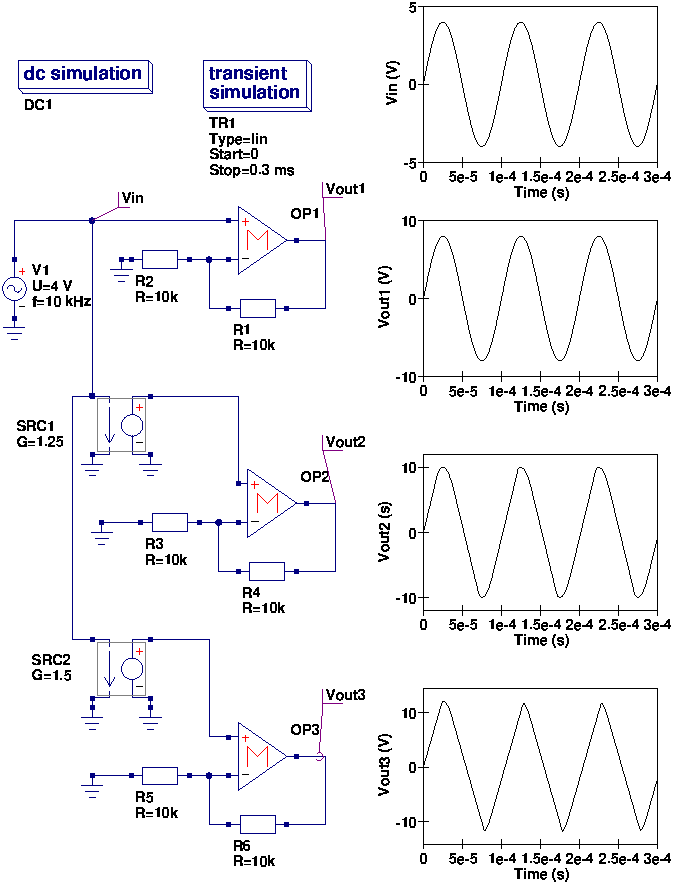
\includegraphics[width=0.7\linewidth]{mod_amp_Fig9}
  \caption{UA741 modular macromodel slewrate limiting test circuit and simulation results}
  \label{fig:mod_amp9}
\end{figure} 


\begin{figure} [here]
  \centering
  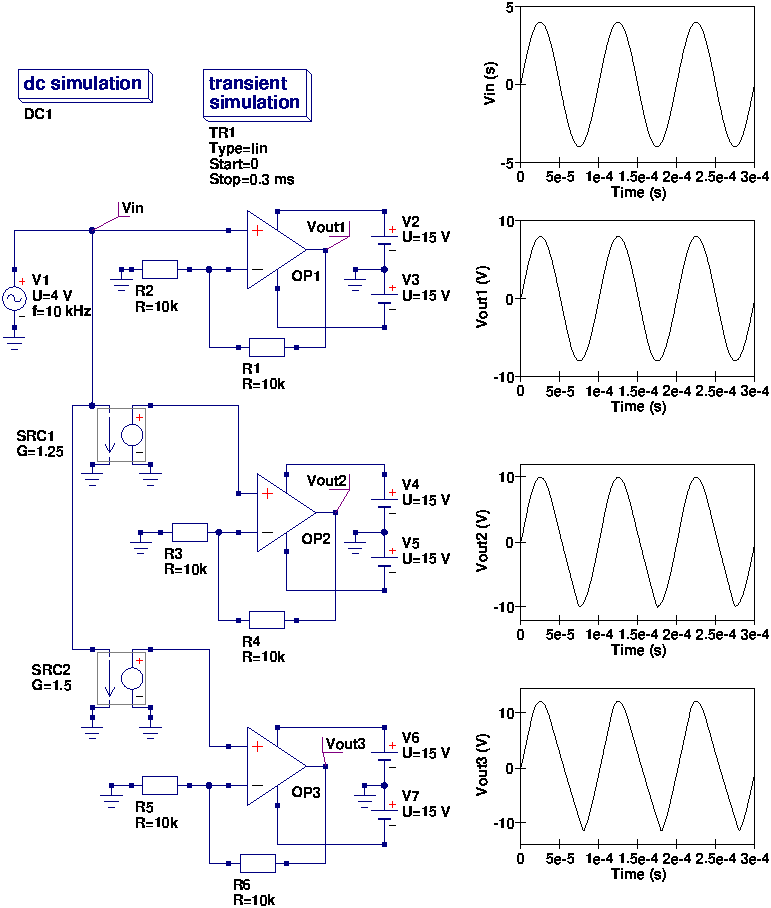
\includegraphics[width=0.7\linewidth]{mod_amp_Fig10}
  \caption{UA741 transistor level slewrate limiting test circuit and simulation results}
  \label{fig:mod_amp10}
\end{figure} 



\tutsection{Output voltage limiting}

Operational amplifier output voltage limiting effects are represented
by the Verilog-A code listed in this section. A Verilog-A if-else
statement is used to model voltage limiting.  This language
construction also demonstrates the use of the Verilog-A block
construction formed with begin-end code words.  Effectively the
if-else statement swaps circuit elements as the voltage signal
polarity changes.  The simulated results for a UA741 voltage limiting
test circuit are illustrated in Figs.~\ref{fig:mod_amp11}
and~\ref{fig:mod_amp12}. Again the results are very similar for both
models. However, in the case of the macromodel there is no attempt to
reduce the differential gain when output voltage limiting occurs and
as a result some waveform distortion takes place.  In practice if, as
in the case of pure AC simulation, output voltage limiting is not
required then simply set VLIMP and VLIMN well outside the range of
required operating voltage and voltage limiting is never triggered.

\begin{lstlisting}[
 language=Verilog, 
 xleftmargin=12pt,
 basicstyle=\scriptsize]
//
// Voltage limiter stage
//
   if (V(out_p) > VLIMP)
      begin
        I(out_p) <+  -10.0*VLIMP;
        I(out_p) <+ 10.0*V(out_p);
      end
  else if (V(out_p) < VLIMN)
      begin
        I(out_p) <+ -10.0*VLIMN;
        I(out_p) <+ 10.0*V(out_p);
     end
  end
\end{lstlisting}

\begin{figure} [here]
  \centering
  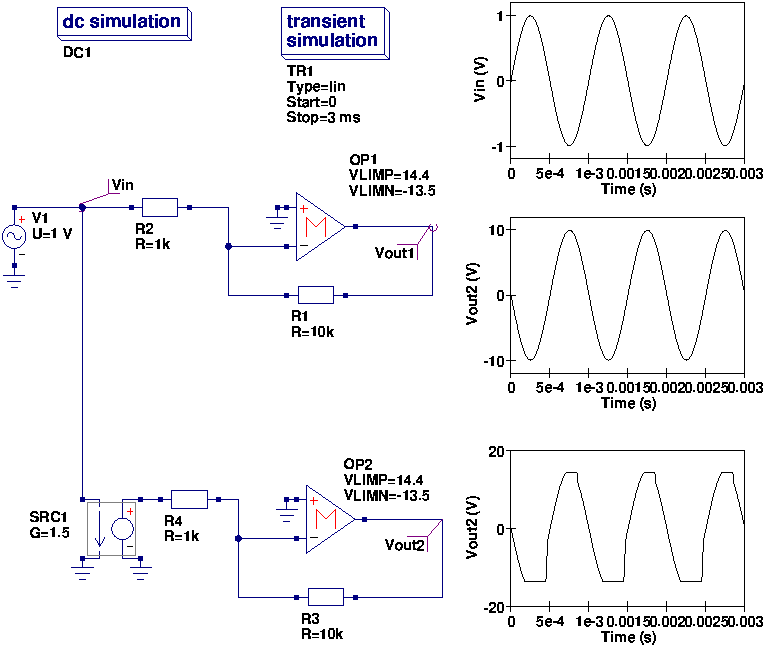
\includegraphics[width=0.75\linewidth]{mod_amp_Fig11}
  \caption{UA741 modular macromodel output voltage limiting test circuit and simulation results}
  \label{fig:mod_amp11}
\end{figure} 


\begin{figure} [here]
  \centering
  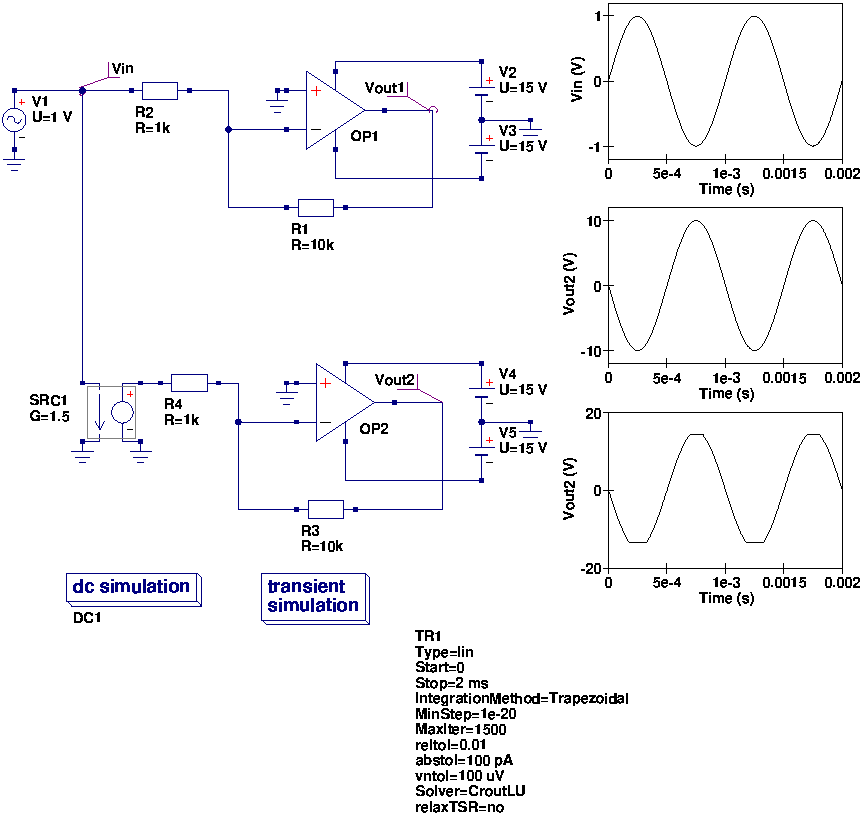
\includegraphics[width=0.8\linewidth]{mod_amp_Fig12}
  \caption{UA741 transistor level output voltage limiting test circuit and simulation results}
  \label{fig:mod_amp12}
\end{figure} 

\tutsection{Output current limiting}

Operational amplifier output current limiting effects are represented
by the Verilog-A code listed in this section. A Verilog-A if-else
statement is used to model current limiting.  The effect is modelled
by a feedback mechanism which reduces the magnitude of current I(n4)
which is proportional to the difference of the current flowing in the
output path and ILMAX.  A scale factor CSCALE is used to adjust
maximum clamped output current.  The simulated results for a UA741
current limiting test circuit are illustrated in
Figs.~\ref{fig:mod_amp14} and~\ref{fig:mod_amp15}. Current clamping
induces distortion in the output waveform. Both the macromodel and the
transistor level model give roughly the same clamped output currents
but the wave shapes, and hence the distortion, are somewhat different.
This is not surprising as the macromodel does not include a mechanism
to control clamping distortion. Setting CSCALE to zero removes the
current limiting process from the operational amplifier macromodel.

\begin{lstlisting}[
 language=Verilog, 
 xleftmargin=12pt,
 basicstyle=\scriptsize]
//
// Current limiter stage
//
   if (V(n2, out_p) >= ILMAX) 
      begin
        I(n4) <+  -V(n5);
        I(n4) <+ CSCALE*V(n5)*(V(n2, out_p) - ILMAX);
        I(n4) <+ V(n4);
      end
   else if (V(n2, out_p) <= -ILMAX)
        begin
         I(n4) <+  -V(n5);
         I(n4) <+ -CSCALE*V(n5)*(V(n2, out_p) + ILMAX);
         I(n4) <+ V(n4);
        end
   else
        begin
            I(n4) <+ -V(n5);
            I(n4) <+  V(n4);
        end
//
\end{lstlisting}

\begin{figure} [here]
  \centering
  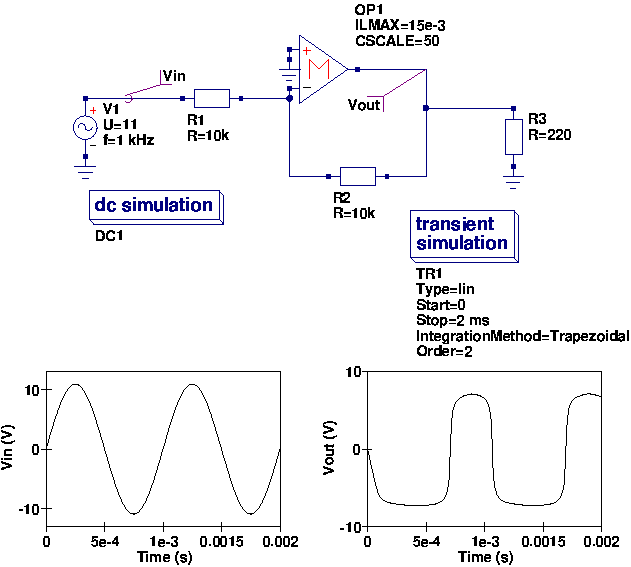
\includegraphics[width=0.75\linewidth]{mod_amp_Fig14}
  \caption{UA741 modular macromodel output current limiting test circuit and simulation results}
  \label{fig:mod_amp14}
\end{figure} 


\begin{figure} [here]
  \centering
  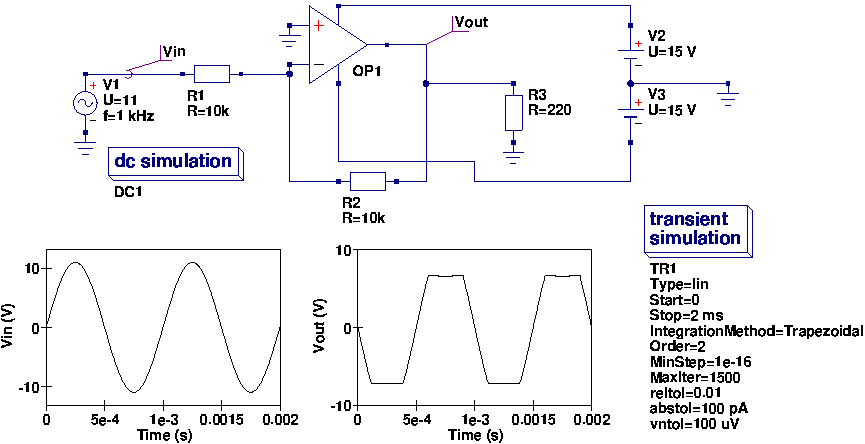
\includegraphics[width=0.85\linewidth]{mod_amp_Fig15}
  \caption{UA741 transistor level output current limiting test circuit and simulation results}
  \label{fig:mod_amp15}
\end{figure} 


\tutsection{End note}

These notes summarise a number of techniques for modelling operational
amplifier functions using Verilog-A.  Verilog-A is primarily intended
for modelling compact semiconductor devices.  However, as this report
demonstrates it can be equally employed for macromodelling of
integrated circuits and circuits in general. The Qucs C++ code for the
modular operational amplifier model, generated by ADMS, can be found
in the Qucs release source tarballs at
\url{http://qucs.sourceforge.net}.  The procedure followed to convert
the Verilog-A code into C++ for compilation and linking with Qucs
closely followed that described by Sefan Jahn and H\'{e}l\`{e}ne
Parruitte.  Although it takes more work to construct models using ADMS
the effort is worthwile because the finished models are very efficient
in terms of memory usage and have significantly reduced run times. One
interesting observation which is worth recording here is the fact that
Qucs equation defined device (EDD) models and ADMS Verilog-A models
have a very similar structure, implying that EDD models can be used as
prototypes prior to compilation and linking via the compact device
modelling route using ADMS. Once again a special thanks to Stefan Jahn
for all his help and encouragement over the period that I have been
developing the Verilog-A version of the operational amplifier
macromodel, writing this report and testing the examples it includes.
